\documentclass[conference]{IEEEtran}
\usepackage[utf8]{inputenc}
\usepackage{mathtools}
\usepackage{amsmath}
\usepackage{graphicx}
\usepackage{float}
\usepackage[italian]{babel}

\setlength{\columnsep}{14mm}

\newcommand{\abs}[1]{\left|#1\right|}

\title{Predizione della struttura di una proteina (PSP) in un lattice 2D}

\author{Emanuele Carraro}

\begin{document}

\maketitle    

\begin{abstract}
{\it Il problema di predizione della struttura terziaria di una proteina è molto rilevante nell'ambito della bioinformatica, infatti la configurazione assunta nello spazio determina le sue proprietà biologiche.

Di seguito vengono analizzati tre metodi di risoluzione del problema, uno tramite ricerca informata (algoritmo hill-climbing), uno tramite la definizione di un problema con vincoli e, infine, uno tramite un noto algoritmo di reinforcement learning (Q-learning).
}
\end{abstract}

\section{Nomenclatura}

\begin{itemize}
 \item PSP Protein structure prediction
 \item $\mathcal{E}_c$ Matrice dell'energia di una proteina
 \item H Amminoacido idrofobico
 \item P Amminoacido polare
 \item $\mathcal{S}$ Spazio degli stati
 \item $\mathcal{A}$ Spazio delle azioni
 \item $\mathcal{R}$ Funzione di ricompensa
 \item $\delta$ Funzione di transizione
\end{itemize}

\section{Background}

Una proteina è un complesso biologico di macromolecole composte da \textbf{sequenze di amminoacidi}.

Gli amminoacidi vengono uniti durante la sintesi proteica grazie alla creazione di un legame peptidico (figura \ref{fig:pept}).

\begin{figure}[h]
\centering
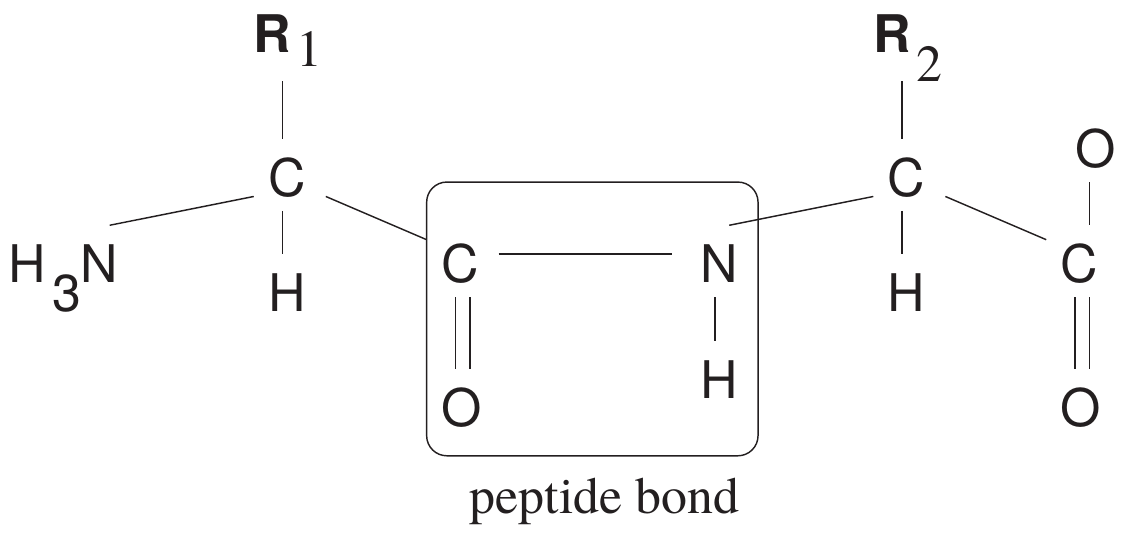
\includegraphics[width=0.4\textwidth]{figure/peptideBond.png}
\caption{Legame peptidico}
\label{fig:pept}
\end{figure}

La \textbf{struttura primaria} di una proteina è data dalla pura sequenza di amminoacidi e condiziona la configurazione spaziale e la forma globale della molecola.

L'avvolgimento a spirale e la disposizione regolare di tratti più o meno lunghi della catena proteica costituiscono la sua \textbf{struttura secondaria}.\\

Di solito, gruppi di queste strutture secondarie si combinano fra loro per formare la \textbf{struttura terziaria}, dalla quale dipendono le proprietà biologiche della molecola. La predizione della struttura di una proteina (PSP) è quindi una sfida molto importante nell'ambito della biologia molecolare.

Le tecniche computazionali di psp assumono che la struttura primaria di una proteina determini completamente la sua struttura terziaria (anche se nella realtà ci sono alcune eccezioni).

I modelli basati sulla struttura \textit{lattice} (o reticolo) si sono dimostrati utili per ragionare a proposito della complessità di questo problema. Un modello con lattice porta a ``discretizzare'' lo spazio di configurazione di una proteina e può essere classificato in base a determinate proprietà:

\begin{enumerate}
 \item Come viene rappresentata la struttura di una proteina? (ad esempio, tramite un grafo)
 \item Quale alfabeto di amminoacidi viene utilizzato? (tutti i 20 conosciuti oppure solo 2 categorie - (H) idrofobi o (P) polari)
 \item Quale formula utilizzare per descrivere l'\textbf{energia di una conformazione}? (equivalente a una funzione di costo in un problema di ottimizzazione)
 \item Che tipo di lattice scegliere) (ad esempio, un lattice quadratico - 2D - o cubico - 3D)
\end{enumerate}

\subsection{Il modello HP}

Uno dei modelli più usati è il modello HP: il lattice usato semplifica la struttura primaria di una proteina in un grafo, dove i nodi sono gli amminoacidi e gli archi sono i legami peptidici. Ogni nodo è un amminoacido che può essere di 2 tipi: H (idrofobico) o P (polare), così la proteina può essere rappresentata tramite una stringa. Si è osservato che in questo modello le proteine tendono a raggruppare i nodi H attorno a un punto (cioè gli amminoacidi idrofobici formano un ``nucleo'') mentre i nodi P rimangono esterni.

Nella seguente notazione si denota H con 1 e P con 0. Una proteina è dunque una sequenza binaria. L'energia usata in questo modello è data dal numero di ``contatti'' tra H (1). Se due amminoacidi H si trovano su punti adiacenti del lattice, allora contribuiscono di un'unità (negativa) all'energia.
Formalmente, sia s una sequenza binaria di dimensioni ($|s|\cdot|s|$) e $\mathcal{E}_c$ la matrice quadrata associata all'energia di una sua configurazione c. Allora, dati due punti a e b della sequenza \textbf{adiacenti nel lattice}, l'energia è definita dalla seguente equazione:

\begin{equation}
    \mathcal{E}_c = (e(a,b))_{a,b \in s} =
    \begin{cases*}
      -1 & se a = b = 1 \\
      0  & altrimenti
    \end{cases*}
\end{equation}

\subsection{Complessità computazionale del problema}

La ricerca esaustiva nello spazio delle possibili configurazioni di una proteina non è una soluzione algoritmica efficiente (non opera in tempo polinomiale) in quanto il numero di possibili configurazioni cresce esponenzialmente in relazione alla lunghezza della proteina.

Eppure, in natura il processo di ``folding'' (ripiegamento) di una proteina accade velocemente (varia da qualche secondo a qualche minuto). L'ipotesi più accreditata è che una proteina assuma la configurazione con energia minima.

Di conseguenza, dato un modello di lattice L e una sequenza s, l'obiettivo è trovare una configurazione c di s senza cicli in L che minimizzi l'energia.

\subsection{Modello square lattice}

Un reticolo a quadrato (square lattice) è un lattice a 2 dimensioni sugli interi ($Z^2$). Considerando un modello square lattice, l'impostazione del problema rimane la stessa, con il vincolo che gli amminoacidi/nodi del grafo debbano essere posizionati solo nei punti del reticolo.

Fornire un upper bound rispetto all'energia è un passo utile nello studio di questo modello. Si cerca qual è il numero massimo di contatti per una configurazione. Sia s una sequenza binaria e siano $\mathcal{P}[s]$ il numero di 1 in posizioni pari e $\mathcal{D}[s]$ il numero di 1 in posizioni dispari.

Dato che questo modello di lattice è bipartito, ogni 1 in posizione pari può avere un contatto con un 1 in posizione dispari. Sia $\mathcal{X}[s] = min\{\mathcal{P}[s], \mathcal{D}[s]\}$ (il minimo numero di 1 in posizione pari/dispari).

In ogni conformazione, il numero di contatti che può avere un 1 nella sequenza che non sia nè all'inizio nè alla fine, è 2 (altrimenti sarebbero 3). Quindi, il numero massimo di contatti in una configurazione di s nel reticolo quadrato è: $2 \mathcal{X}[s] + 2$ (un esempio è riportato in figura \ref{fig:optConfig})

\begin{figure}[h]
\centering
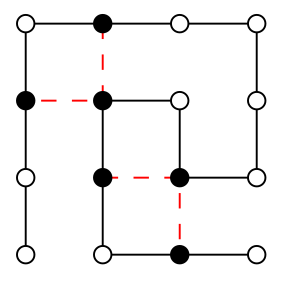
\includegraphics[width=0.3\textwidth]{figure/optConfig}
\caption{Una configurazione ottima per la sequenza 0010100001011010. I punti neri rappresentano 1 (H) mentre i punti bianchi 0 (P). Questa configurazione ha 4 contatti (linee tratteggiate) quindi l'energia totale è -4. L'upper bound per il numero massimo di contatti in questa sequenza è 2*2 + 2 = 6 ($\mathcal{X}[s] = 2$) \dots questo rappresenta un upper bound sul numero di contatti, non l'ottimo}
\label{fig:optConfig}
\end{figure}

\section{Problema con vincoli}

Data la struttura primaria di una proteina di lunghezza n, un problema tramite vincoli si definisce nel seguente modo:

\begin{enumerate}
 \item ciascun amminoacido viene assegnato a un punto sul reticolo 2D di dimensione $n \cdot n$ ($(x_i, y_i) \in Z^2$ $\forall i \in 1,..,n$, le coordinate i-esime appartengono all'amminoacido i-esimo);
 \item punti successivi nella struttura primaria non possono essere a una distanza maggiore di 1 tra loro ($\abs{x_i - x_{i+1}} + \abs{y_i - y_{i+1}} = 1 $ $\forall i \in 1,..,n-1$);
 \item due amminoacidi distinti non possono essere assegnati allo stesso punto sul reticolo ($ \neg (x_i = x_j \land y_i = y_j)$ $\forall i,j \in 1,..,n$).
\end{enumerate}

L'insieme di queste condizioni fa sì che il problema con vincoli ritorni l'intero insieme di configurazioni ammissibili della proteina nel reticolo 2D. Molte di queste sono ``simmetriche'', ossia la configurazione rimane la stessa ma la catena viene ``srotolata'' al contrario. Nella valutazione delle soluzioni non si tiene conto di queste simmetrie. Il problema così definito ritorna un insieme numeroso di soluzioni, esponenziale rispetto alla dimensione dell'input.

\section{Hill climbing search}

La hill climbing search necessita di:

\begin{enumerate}
 \item un modo per rappresentare una soluzione;
 \item una soluzione iniziale;
 \item una definizione di vicinato (come ci si sposta da una soluzione a una sua ``vicina''?);
 \item una funzione che valuti le soluzioni;
 \item una strategia di esplorazione.
\end{enumerate}

L'implementazione della hill climbing search è avvenuta nel seguente modo:

\begin{enumerate}
 \item una soluzione è data da un vettore di interi, uno per ogni amminoacido. Ciascun intero rappresenta la posizione di un amminoacido nella configurazione (una matrice quadrata). Per essere ammissibile, la soluzione non deve avere cicli nè salti (parti staccate).
 \item una soluzione iniziale è una soluzione scelta in modo random
 \item la definizione di vicinato in questo caso ha una forte componente randomica: data una soluzione, la struttura viene ``rotta'' in un punto casuale tra l'inizio e la fine della configurazione e da quel punto si scelgono mosse diverse (randomiche), determinando così il vicino. In questo modo, se il punto di taglio viene scelto all'inizio, gran parte della configurazione viene persa (al contrario, la maggior parte viene mantenuta).
 \item come funzione di valutazione delle soluzioni viene usata l'\textbf{energia di una configurazione} $\mathcal{E}_c$
 \item come strategia di esplorazione del vicinato viene usata la \textbf{best-first strategy}
\end{enumerate}

\section{Reinforcement Learning}

Un task di reinforcement learning è composto da:

\begin{enumerate}
 \item lo spazio degli stati $\mathcal{S}$;
 \item lo spazio delle azioni $\mathcal{A}$;
 \item la funzione di transizione $\sigma$ che mappa una coppia (stato, azione) a uno dei probabili stati successori;
 \item la funzione di ricompensa;
\end{enumerate}

Lo spazio degli stati $\mathcal{S}$ consiste di $\frac{4^n - 1}{3}$ ed è rappresentato in figura \ref{fig:stateSpace}.

\begin{figure}[h]
\centering
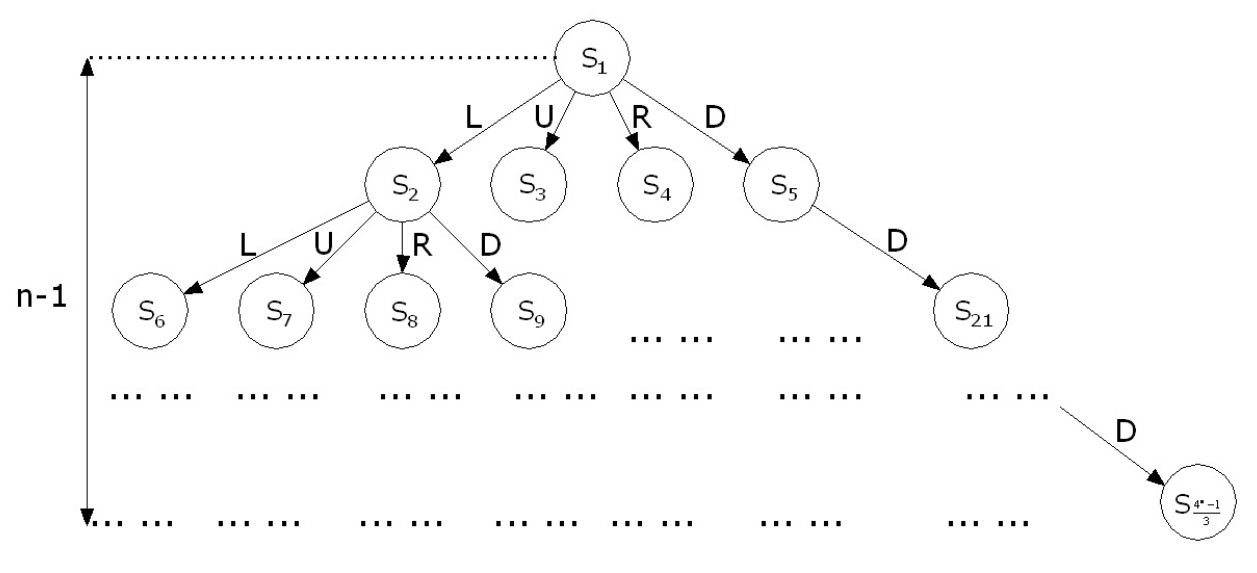
\includegraphics[width=0.5\textwidth]{figure/stateSpace.png}
\caption{Spazio degli stati per il task di reinforcement learning}
\label{fig:stateSpace}
\end{figure}

Ciascuno stato è collegato a 4 vicini tramite 4 possibili azioni: $\mathcal{A} = \{ L, R, U, D\}$; L (left) $a_1$, R (right) $a_2$, U (up) $a_3$, D (Down) $a_4$.

\subsection{Funzione di transizione}

La funzione di transizione è un caso particolare applicato a un albero con fattore di ramificazione 4.

In generale, dato un albero T con fattore di ramificazione b, un nodo/stato i e un'azione (ramo) a, il nodo/stato di arrivo j è dato dalla formula:

\begin{equation}
j = i + b*pn + sn + a
\end{equation}

dove pn sono i nodi precedenti a i e sn sono i nodi successivi. Ricordando che pn è pari al numero di nodi totali del livello (nt) meno quelli successivi e i (pn = nt - sn - 1), l'indice dello stato di arrivo è dato dalla seguente formula:

\begin{equation}
j = b*i + a - b + 1
\end{equation}

I calcoli sono stati sviluppato in appendice (\ref{appendix:sviluppo}).

Dunque per b = 4, la formula diventa:

\begin{equation}
\tag{Funzione di transizione}
4i + a - 3
\end{equation}

La funzione di transizione, dato uno stato $s_i$ e un'azione $a_k$ è definita dalla formula:

\begin{equation}
\delta(s_i, a_k) = s_{4*i - 3 + k} \forall k \in [1,4] \qquad \forall i 1 \leq i \leq \frac{4^n - 1}{3}
\end{equation}

La funzione di ricompensa è definita da [Czibula et al.] nel paper ``A Reinforcement Learning Model for Solving the Folding Problem'' nel modo seguente:

\begin{equation}
    \label{eq:rew}
    \mathcal{R}(\pi_k| s_1, \pi_1, \pi_2, \dots \pi_{k-1}) =
    \begin{cases*}
      0.01 & se $a_{\pi}$ non è valida \\
      - E_{\pi} & se k = n - 1 \\
      0.1 & altrimenti
    \end{cases*}
\end{equation}

dove $\pi_k$ è lo stato finale dato dal percorso $\pi = (s_1, \pi_1, \pi_2, \dots \pi_{k-1})$ e $a_{\pi}$ denota la sequenza di azioni che hanno portato allo stato $\pi_k$ a partire da $s_1$. Una sequenza di azioni si dice valida se produce una configurazione senza cicli. $E_{\pi}$ è l'energia data dalla configurazione ottenuta in $\pi_k$ tramite la sequenza $a_{\pi}$.

Ho scelto di testare una versione alternativa della funzione di ricompensa nel caso in cui l'azione $a_{\pi}$ non sia valida: a mio parere una ricompensa di 0.01 (per quanto piccola) può far deviare l'agente in fase di test verso cammini che conducono a una sequenza non valida. Ho quindi cambiato il segno della ricompensa per renderla negativa (-0.01) e penalizzare l'agente.

Il task di reinforcement learning deve allenare un agente nel trovare un percorso $\pi$ che porti a uno stato finale in cui l'energia associata sia minima.

\subsection{Obiettivo}

In ogni istante t, l'agente osserva uno stato e decide un'azione da intraprendere, che lo sposta nello stato successivo ricevendo una ricompensa $r_t$. Il suo obiettivo è massimizzare la somma attesa delle ricompense che ottiene:

\begin{equation}
\mathcal{E}[\mathcal{R}] = r_0 + \gamma*r_1 + \gamma^2*r_2 + \dots.
\end{equation}

In questo caso l'energia è data con segno opposto (per minimizzarla effettivamente).

L'agente può esplorare o avere una strategia greedy. Nella fase di training sarà necessario esplorare molto così da capire quali azioni danno maggior ricompensa.

Esistono 2 modi che l'agente ha per imparare una propria strategia:

\begin{enumerate}
 \item l'agente impare una funzione di utilità per ogni stato e la usa per selezionare le azioni
 \item l'agente impara una funzione Q di utilità per ogni coppia (stato, azione) così da selezionare in ogni stato l'azione appropriata
\end{enumerate}

La seconda modalità viene chiamata Q-learning ed è quella che ho scelto di implementare secondo la definizione descritta da [Czibula et al.] nel paper ``A Reinforcement Learning Model for Solving the Folding Problem''

\subsection{Q-Learning}

Il Q-learning considera coppie (stato s, azione a) per ciascuna delle quali è associato un valore (Q-value).

Il Q-value è la somma delle ricompense (possibilmente ridimensionate rispetto a un fattore di sconto $\gamma$) ottenute dall'eseguire l'azione a sullo stato s e proseguendo con una politica data (ad esempio greedy o $\epsilon$-greedy).

Un valore ottimale $Q^*$ è la somma delle ricompense ottenute applicando a su s e proseguendo con la politica ottimale.

L'equazione \ref{eq:q} è stata proposta da [Czibula et al.] e mostra quanto detto: $r(s,a)$ è la ricompensa ottenuta applicando a su s mentre $\gamma * max_{a'} Q(s', a')$ rappresenta le ricompense future moltplicate per un fattore di sconto $\gamma$.

\begin{equation}
\label{eq:q}
Q(s,a) = r(s,a) + \gamma * max_{a'} Q(s', a')
\end{equation}

Gli autori del paper ``A Reinforcement Learning Model for Solving the Folding Problem'' usano l'equazione \ref{eq:q} e la funzione di ricompensa \ref{eq:rew} nella fase di training per aggiornare i valori di Q. Inoltre assumono che:

\begin{itemize}
 \item per ogni coppia (stato s, azione a), Q(s,a) sia pari a 0.
 \item il fattore di sconto $\gamma$ sia 0.9
 \item il numero di episodi sia 36
 \item la politica utilizzata sia greedy ($\epsilon-greedy, \epsilon = 1$)
\end{itemize}

Assumono anche che le coppie (stato, azione) siano visitate uniformemente.

Con questa procedura hanno dimostrato matematicamente che i valori di Q convergerebero ai loro valori ottimali (cioè valori che conduconol'agente alla politica ottimale, corrispondente alla struttura bidimensionale della proteina con minor energia) se si visitassero infinitamente tutte le coppie (stato, azione).

Formalmente, gli autori hanno dimostrato che dato $Q_n(s, a)$ (la stima di $Q(s,a)$ all'n-esimo episodio di training), il limite $\lim_{n \to \infty} Q_n (s,a)$ vale $Q^*(s,a) \quad \forall s \in S, a \in A$

\section{Analisi}

Gli autori utilizzano una politica strettamentre esplorativa in fase di training ($\epsilon-greedy, \epsilon = 1$), quindi permettono di esplorare lo spazio degli stati uniformemente.

Una possibile modifica potrebbe essere abbassare $\epsilon$ da 1 a (ad esempio) 0.6 e rendere il training epsilon-greedy.

Inoltre il numero di episodi è molto piccolo: 36 può essere sufficiente per l'esempio riportato dagli autori (HHPH), ma per proteine più lunghe serve un maggior numero di episodi.

I risultati riportati nel paper sono discutibili in quanto non viene specificato nessun seed e nemmeno quante volte è stato eseguito l'algoritmo. In particolare, riportare la tabella dei valori Q non è molto utile, dato che vengono trovati in fase di training che è prettamente esplorativa: senza un seed i valori sono impossibili da riprodurre.

\section{Test e risultati}

\textbf{Nota}: per la hill climbing search  e il q learning vengono riportati il numero minimo di iterazioni ed episodi (rispettivamente) con cui sono stati raggiunti i risultati riportati.

I test vengono eseguiti su 5 proteine di lunghezze diverse (4, 9, 16, 20, 36):

\begin{itemize}
 \item p4 = HHPH
 \item p9 = HPHHPHHPH
 \item p16 = PPHPHPPPPHPHHPHP
 \item p20 = HPHPPHHPHPPHPHHPPHPH
 \item p36 = PPPHHPPHHPPPPPHHHHHHHPPHHPPPPHHPPHPP
\end{itemize}

Vengono variati 3 seed e infine viene eseguito un test in modo totalmente random. Durante i test il limite massimo di iterazioni è fissato per tutti i seed nel seguente modo: p4 - 50 it, p9 - 200 it, p16 - 500 it, p20 - 1000 it, p36 - 2000 it. Se in nessun caso si è raggiunto un risultato entro il numero massimo di iterazioni, allora la tabella dei risultati non viene riportata e ciò significa che il tempo richiesto è probabilmente maggiore (ad esempio nel test del Q-Learning v-paper per la sequenza p36).

\subsection{Test per problema con vincoli}

\begin{table}[H]
\begin{center}
\begin{tabular}{|c|c|c|}
\hline
\textbf{Proteina} & \textbf{Tempo (s)} & \textbf{Energia} \\ \hline
p4 & 0.0346564320007019 & -1 \\ \hline
p9 & 8.78769836499987 & -3 \\ \hline
\end{tabular}
\end{center}
\caption{Risultati tramite problema con vincoli}
\end{table}

\subsection{Test per hill climbing search}

\begin{table}[h]
\begin{center}
\begin{tabular}{|c|c|c|c|c|}
\hline
\textbf{Seed} & \textbf{\# interazioni} & \textbf{Tempo (s)} & \textbf{Energia} \\ \hline
3 & 2 & 0.00049901008606 & -1 \\ \hline
1234 & 2 & 0.000531911849976 & -1 \\ \hline
42 & 2 & 0.00047492980957 & -1 \\ \hline
random (figura \ref{fig:lsp4}) & 2 & 0.000494003295898 & -1 \\ \hline
\end{tabular}
\end{center}
\caption{Risultati tramite hill climbing search per p4}
\end{table}

\begin{figure}[H]
\centering
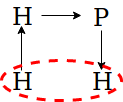
\includegraphics[width=0.10\textwidth]{figure/p4LS.png}
\caption{Hill climbing search - p4 (random)}
\label{fig:lsp4}
\end{figure}

\begin{table}[H]
\begin{center}
\begin{tabular}{|c|c|c|c|c|}
\hline
\textbf{Seed} & \textbf{\# interazioni} & \textbf{Tempo (s)} & \textbf{Energia} \\ \hline
3 & 4 & 0.00353193283081 & -3 \\ \hline
1234 & 3 & 0.00242280960083 & -3 \\ \hline
42 (figura \ref{fig:lsp9}) & 2 & 0.00117897987366 & -3 \\ \hline
random & 3 & 0.00240302085876 & -3 \\ \hline
\end{tabular}
\end{center}
\caption{Risultati tramite hill climbing search per p9}
\end{table}

\begin{figure}[H]
\centering
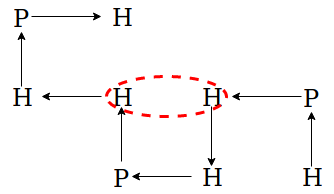
\includegraphics[width=0.25\textwidth]{figure/p9LS.png}
\caption{Hill climbing search - p9 (seed 42)}
\label{fig:lsp9}
\end{figure}

\begin{table}[H]
\begin{center}
\begin{tabular}{|c|c|c|c|c|}
\hline
\textbf{Seed} & \textbf{\# interazioni} & \textbf{Tempo (s)} & \textbf{Energia} \\ \hline
3 & 47 & 0.150655031204 & -4 \\ \hline
1234 & 33 & 0.0698339939117 & -4 \\ \hline
42 & 228 & 1.0661611557 & -4 \\ \hline
random (figura \ref{fig:lsp16}) & 12 & 0.0363581180573 & -4 \\ \hline
\end{tabular}
\end{center}
\caption{Risultati tramite hill climbing search per p16}
\end{table}

\begin{figure}[H]
\centering
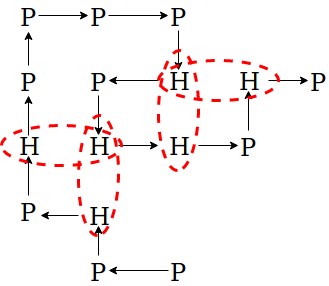
\includegraphics[width=0.25\textwidth]{figure/LSP16.png}
\caption{Hill climbing search - p16 (random)}
\label{fig:lsp16}
\end{figure}

\begin{table}[H]
\begin{center}
\begin{tabular}{|c|c|c|c|c|}
\hline
\textbf{Seed} & \textbf{\# interazioni} & \textbf{Tempo (s)} & \textbf{Energia} \\ \hline
3 & 741 & 2.14663600922 & -7 \\ \hline
1234 & 854 & 2.94443798065 & -8 \\ \hline
42 & 250 & 0.715470075607 & -8 \\ \hline
random & 88 & 0.25554394722 & -9 \\ \hline
\end{tabular}
\end{center}
\caption{Risultati tramite hill climbing search per p20}
\end{table}

\subsection{Test per Q-learning}

\begin{table}[H]
\begin{center}
\begin{tabular}{|c|c|c|c|c|}
\hline
\textbf{Seed} & \textbf{\# episodi} & \textbf{Tempo (s)} & \textbf{Energia} \\ \hline
3 & 9 & 0.000707149505615 & -1 \\ \hline
1234 & 39 & 0.00345897674561 & -1 \\ \hline
42 & 9 & 0.000800132751465 & -1 \\ \hline
random & 1 & 2.21729278564e-05 & -1 \\ \hline
\end{tabular}
\end{center}
\caption{Risultati tramite Q-learning [v. paper] per p4}
\end{table}

\begin{table}[H]
\begin{center}
\begin{tabular}{|c|c|c|c|c|}
\hline
\textbf{Seed} & \textbf{\# episodi} & \textbf{Tempo (s)} & \textbf{Energia} \\ \hline
3 & 26 & 0.00551986694336 & -2 \\ \hline
1234 & 11 & 0.00375199317932 & -1 \\ \hline
42 & 74 & 0.0227060317993 & -2 \\ \hline
random & 26 & 0.0056300163269 & -2 \\ \hline
\end{tabular}
\end{center}
\caption{Risultati tramite Q-learning [v. paper] per p9}
\end{table}

\begin{table}[H]
\begin{center}
\begin{tabular}{|c|c|c|c|c|}
\hline
\textbf{Seed} & \textbf{\# episodi} & \textbf{Tempo (s)} & \textbf{Energia} \\ \hline
3 & >500 & - & - \\ \hline
1234 & >500 & - & - \\ \hline
42 & >500 & - & - \\ \hline
random & 254 & 0.195900917053 & -1 \\ \hline
\end{tabular}
\end{center}
\caption{Risultati tramite Q-learning [v. paper] per p16}
\end{table}

\begin{table}[H]
\begin{center}
\begin{tabular}{|c|c|c|c|c|}
\hline
\textbf{Seed} & \textbf{\# episodi} & \textbf{Tempo (s)} & \textbf{Energia} \\ \hline
3 & 52 & 0.0305478572845 & -1 \\ \hline
1234 & >1000 & - & - \\ \hline
42 & >1000 & - & - \\ \hline
random & 822 & 0.513980150223 & -2 \\ \hline
\end{tabular}
\end{center}
\caption{Risultati tramite Q-learning [v. paper] per p20}
\end{table}

\appendix
\label{appendix:sviluppo}

\begin{equation}
\begin{split}
j   & = i + b(nt - sn - 1) + \bigg(\frac{b^{l + 1} - 1}{b - 1} - i\bigg) + a\\
    & = i + b(nt - sn - 1) + \bigg(\frac{b^{l + 1} - 1}{b - 1} - i\bigg) + a\\
    & = i + b\bigg(b^{l} - \frac{b^{l + 1} - 1}{b - 1} + i - 1\bigg) + \frac{b^{l + 1} - 1}{b - 1} - i + a\\
    & = b\bigg(b^{l} - \frac{b^{l + 1} - 1}{b - 1} + i - 1\bigg) + \frac{b^{l + 1} - 1}{b - 1} + a\\
    & = b^{l + 1} - b\bigg(\frac{b^{l + 1} - 1}{b - 1}\bigg) + bi -b + \frac{b^{l + 1} - 1}{b - 1} + a\\
    & = b^{l + 1} - \frac{b^{l + 2} - b}{b - 1} + bi -b + \frac{b^{l + 1} - 1}{b - 1} + a\\
    & = b^{l + 1} + \frac{b - b^{l + 2}}{b - 1} + bi -b + \frac{b^{l + 1} - 1}{b - 1} + a\\
    & = \frac{b^{l + 1}(b - 1) + b - b^{l + 2} + bi(b - 1) -b^2 + b + b^{l + 1} - 1}{b - 1} + a\\
    & = \frac{b^{l + 2} - b^{l + 1} + b - b^{l + 2} + b^2i - bi -b^2 + b + b^{l + 1} - 1}{b - 1} + a\\
    & = \frac{b^2i - bi - b^2 + 2b - 1}{b - 1} + a\\
    & = \frac{bi(b - 1) - (b^2 - 2b + 1)}{b - 1} + a\\
    & = \frac{bi(b - 1) - (b - 1)^2}{b - 1} + a\\
    & = \frac{(b -1)(bi - b + 1)}{b-1} + a\\
    & = bi + a - b + 1
\end{split}
\end{equation}

\end{document}
